\documentclass[10pt,twocolumn,letterpaper]{article}

%-----------------------------------------------------------------------------------------------------------------------
% Packages
%-----------------------------------------------------------------------------------------------------------------------

\usepackage{cvpr}
\usepackage{times}
\usepackage{epsfig}
\usepackage{graphicx}
\usepackage{amsmath}
\usepackage{amssymb}
\usepackage{algorithm}
\usepackage[noend]{algpseudocode}
\usepackage{float}
\usepackage{subcaption}

% All packages must be included before hyperref
\usepackage[breaklinks=true,bookmarks=false]{hyperref}

%-----------------------------------------------------------------------------------------------------------------------
% Settings
%-----------------------------------------------------------------------------------------------------------------------

% Indicates this is the final version of the CVPR paper, and the paper ID.
\cvprfinalcopy
\def\cvprPaperID{****}

% Improve the boxes around links and references.
\def\httilde{\mbox{\tt\raisebox{-.5ex}{\symbol{126}}}}

% Pages are numbered in submission mode, and unnumbered in camera-ready
\setcounter{page}{1}

%-----------------------------------------------------------------------------------------------------------------------
% Title and Authors
%-----------------------------------------------------------------------------------------------------------------------

\begin{document}

\title{Thick-Edge Polygonal Approximation for Object Tracking}

\author{
    Brandon Perez \\
    Carnegie Mellon University \\
    \textit{\small bmperez@andrew.cmu.edu} \\
    \and
	Sohil Shah \\
    Carnegie Mellon University \\
    \textit{\small sohils@andrew.cmu.edu} \\
}

\maketitle

%-----------------------------------------------------------------------------------------------------------------------
% Abstract
%-----------------------------------------------------------------------------------------------------------------------

\begin{abstract}
    In this paper, we outline a pipeline to approximate moving objects with simple polygons using thick-edge polygonal
    approximation. Simple polygons are easier to use for high computational tasks such as object tracking, since there
    are a fewer number of points to track. We first use a multiple-cue based background subtraction method to detect
    foreground objects in the image and then convert it into a foreground mask. This mask will be used as a binary image
    input to a contour detection algorithm. By creating an accurate polygon approximation, we can represent the object
    more effectively than with simple bounding box, more information is retained. Our results show the representation
    maintains more shape information than simpler approaches such as the Ramer-Douglas-Puecker algorithm while still
    being fast and significantly reducing the number of vertices. We also show success in real surveillance data as well
    as a live webcam feed of soft and rigid bodies.
\end{abstract}

%-----------------------------------------------------------------------------------------------------------------------
% Introduction and Motivation
%-----------------------------------------------------------------------------------------------------------------------

\section{Introduction}

Polygonal approximation seeks to find a reasonable approximation of the input polygon, preserving its shape while
reducing the number of vertices used to represent the polygon. More generally, this applies to contours, which are often
also referred to as polylines. A polygon is a closed contour, or closed polyline.

In particular, the approximation approaches are interested in finding the minimum number of \textit{dominant points}
needed to represent a polygon. A dominant point is defined as the point with maximum local curvature on a given contour.

\subsection{Feature Detection Approaches}

One approach to approximating a contour is find the dominant points by using a feature detector. Typically, some variant
of a corner detector is used. The idea is that since we are looking for a point with maximal curvature, a corner should
be a dominant point as it has a high curvature. The gradients of these points are used to compute their curvature, and
similar to regular corner detection, non-maximum suppression is used to filter out redundant points \cite{Teh1989}.

\subsection{Polygonal Approximation Approaches}

The other class of approaches to approximating a contour are the polygonal approximation approaches. These focus on
using properties of the contour to determine the dominant points and which points should be kept for a good
approximation. For example, some approaches focus on minimizing the deviation of the points from approximated polygon's
border \cite{Ramer1972}. Others focus on minimizing the deviation of area per unit length of the approximated polygon
\cite{Wall1984}.

\subsection{Thick-Edge Polygonal Approximation}

A drawback to both feature detection approaches and most polygonal approximation approaches is that they have a
difficult time with bumpy contours. For feature detection approaches, they tend to generate far too many dominant points
for a compact representation. For polygonal approximation approaches, they tend to miss the finer details of the bumpy
contour, generating too few points for a good approximation.

The method that we focus on is a recent polygonal approximation approach by Saha et al. \cite{Saha2017} that addresses
these issues with bumpy contours. Like other polygonal approximation methods, this is a divide and conquer recursive
method. The algorithm focuses on thickness of points along the contours, similar to the deviation of the points from the
approximated polygon's border. The algorithm has a user controlled thickness parameter that ensures the polygon's points
do not deviate from the approximation by more than that amount, ensuring a good approximation even with bumpy contours.

\subsection{Background Subtraction}

Background subtraction is an algorithm in computer vision that removes the background from a video sequence with a
moving foreground image. This is a very important technique in automated surveillance as it isolates moving objects for
further processing or analysis. For example, it might isolate moving cars and ignore the road and trees. This is useful
in applications such as counting the number of cars passing a particular point, or detecting car accidents. For the
purpose of estimating moving objects with polygons, background subtraction is important in forming a binary image of the
moving blob that can then be used to extract a polygon from. There are multiple different algorithms used for background
subtraction, from the very simple frame difference to more sophisticated neural networks. We analyzed multiple methods
for our application to determine the ideal algorithm based on local pixel texture and color cues.

\section{Motivation}

Generally, Computer Vision researchers have been interested in extracting and using the shape of an object. However,
since contours can be very complex, they can requires hundreds to thousands of points to represent. Thus, researchers
have also been interested in effective ways to approximate polygons to represent the shape of an object. The shape of
object is generally a good discriminant, as the shapes of objects tend to be unique, so they can be useful for both
classification and tracking.

In particular, we are interested in approximating the shape of an object to augment object tracking. To represent the
shape of an object, there are two general approaches. The first, pictured in figure \ref{fig:bounding_box_example}, is
to use a  bounding box that encloses the object. The issue with this approach is that, while it is a simple
representation, it is not very accurate, and it captures a lot of the image background. The second approach, pictured in
figure \ref{fig:edge_image_example}, is to use an edge image to find the exact contour around an object. While this
approach is very accurate, the representation is very complex, requiring a great number of points. We use an existing
polygonal approximation approach to strike a balance between these two extremes, providing a good representation of an
object's shape that doesn't require an excessively complex representation.

\begin{figure}
    \centering
    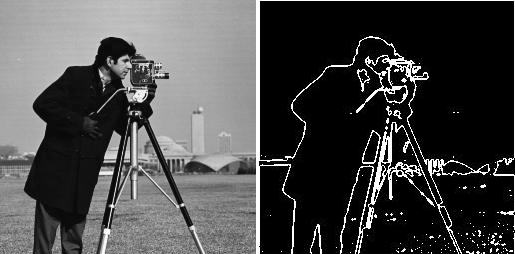
\includegraphics[width=0.495\textwidth]{images/edge_image_example}
    \caption{Example Image and Corresponding Edge Image}
    \label{fig:edge_image_example}
\end{figure}

\begin{figure}
	\centering
    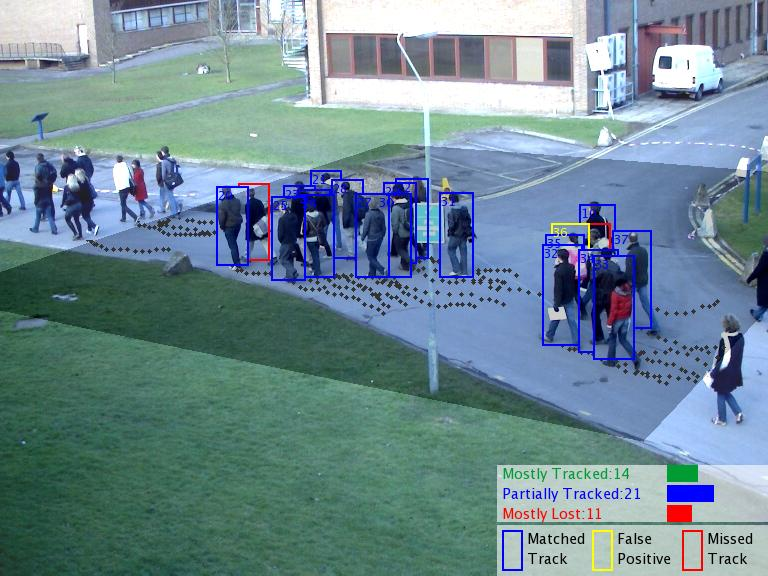
\includegraphics[width=0.495\textwidth]{images/bounding_box_example}
	\caption{Example Image with Bounding Boxes}
	\label{fig:bounding_box_example}
\end{figure}

Our goal is to create a pipeline that can extract the moving objects from a video sequence, find their shapes, and then
compute an effective approximation of the polygon that represents their shape. This approximated representation can be
used by a downstream object tracking pipeline. There are variants of the classic Lucas-Kanade algorithm that use object
contours to augment the tracking algorithm. For example, a  Lucas-Kanade variant proposed by Yilmaz et al.
\cite{Yilmaz2004} uses contours track objects that undergo nonrigid motion. Liu et al. \cite{Liu2006} use a different
tracking algorithm, but use contours to track textureless objects, as the traditional corner features have issues with
these objects.

%-----------------------------------------------------------------------------------------------------------------------
% Related Work
%-----------------------------------------------------------------------------------------------------------------------

\section{Related Work}

\begin{figure*}
	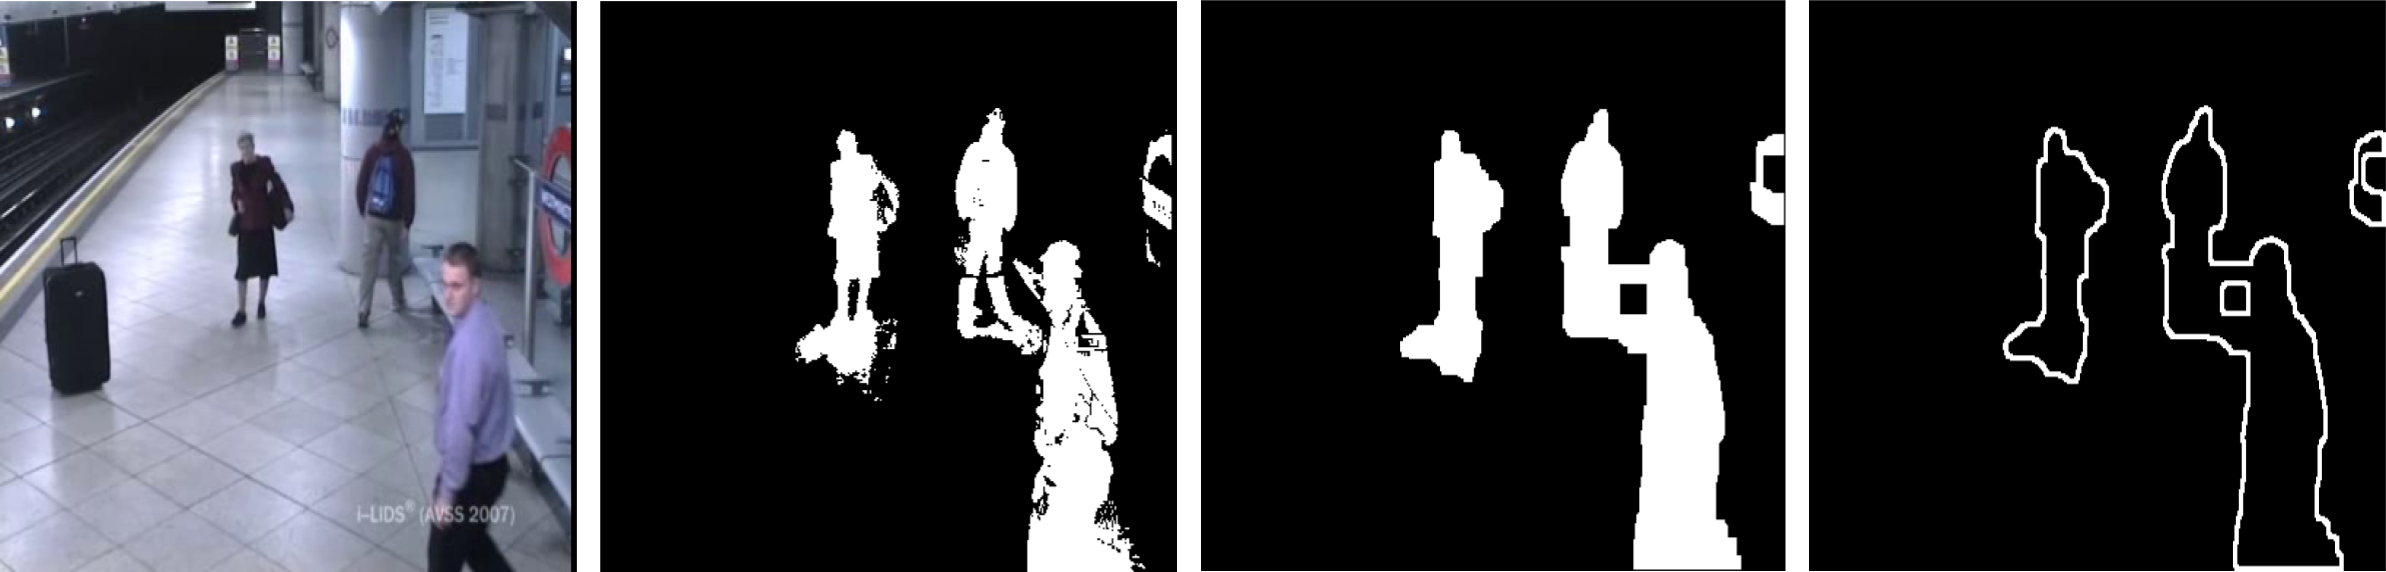
\includegraphics[width=\textwidth]{images/vision_pipeline}
    \caption{Pre-processing flow: first step is to perform background subtraction using the multi-cue model algorithm.
            Next step is to process the image to reduce noise via erosions and dilation. Finally we get closed edges
            using Canny edge detector and contour analysis. This complex contour polygon is then simplified via the
            thick edge polygon approximation.}
	\label{fig:pipeline}
\end{figure*}

\subsection{Ramer-Douglas-Peucker Algorithm}

By far, the most popular and well known polygonal approximation approach is the Ramer-Douglas-Peucker algorithm. This is
a greedy divide and conquer algorithm originally proposed by Ramer \cite{Ramer1972}. The algorithm considers all of the
points between the starting and ending point. First, it marks the endpoints as dominant points, then it finds the point
that is maximally distant from the line between the endpoints. If this exceeds the threshold, then this point is marked
as a dominant point, and all the points are partitioned into two sets based on this point. The algorithm then
recursively processes these two partitions. Otherwise, the points in between the endpoints are discarded.

\subsection{Wall and Danielsson Algorithm}

Another approach was developed by Wall and Danielsson \cite{Wall1984}. This is a sequential approach for partitioning a
polyline. The algorithm focuses on the area per unit length for line segments. This algorithm starts at the beginning
point of the contour. At each step, it adds the next point in contour to the current line segment and computes the area
per unit length of this line segment. Once this exceeds a user defined threshold, the two endpoints of the current line
segment are marked as dominant points, and all points in between are dropped. Then, the algorithm starts a new line
segment at the next point.

%-----------------------------------------------------------------------------------------------------------------------
% Method
%-----------------------------------------------------------------------------------------------------------------------
\section{Approach and Algorithm}

\subsection{Input Data}

The input data used to feed the pipeline was obtained from three different sources. First, the background subtraction
and preprocessing for contour extraction was tested using surveillance data of cars and people at a train station. Next,
the thick-edge polygonal approximation was tested using the MPEG-7 Shape dataset \cite{MPEG-7} of binary polygonal
images. Once these were both verified, the full system was tested together on the surveillance data. After some
fine-tuning, it was finally tested on a live video feed from a webcam.

There were two videos in the surveillance dataset. The first video was of cars traveling in an intersection taken from
the sample datasets of the background subtraction library \cite{bgslibrary}. The video consists of cars moving in a
diagonal line on a highway. There are either zero cars, one car, or multiple cars at any one point in the video, helping
to test lack of movement, single simple movement, and multiple distinct object movement and segmentation.

The second video was from the Advanced Video and Signal based Surveillance conference in London 2007 using surveillance
footage at a train station where subjects abandon their baggage \cite{train_data}. This is a good test of tracking in
simple polygons the complex shape of humans and soft bodies as opposed to cars, whose shapes do not change. Figure
\ref{fig:pipeline} shows an example scene from this dataset and is used to demonstrate the performance of the
preprocessing pipeline.

\subsection{Multi-Cue Background Subtraction}

The background subtraction pipeline uses an open source background subtraction library that implements many different
algorithms \cite{bgslibrary}. We tested each of these methods with live webcam data to select the one that performed the
best empirically. The chosen method is multi-cue background subtraction, described by Noh and Jeon \cite{Noh2013}. This
method performs background subtraction via multiple cues: pixel texture, pixel color, and pixel region. The texture and
location information is used to detect initial foreground and is refined via pixel color. By combining all three methods
to predict a blob for moving objects, this method performs very well on human and vehicle data, especially for the
purpose of automated surveillance. Therefore, we use this method as the starting point of our processing pipeline. An
example of this is seen as the second image of Figure \ref{fig:pipeline}.

\subsection{Contour Extraction}

Once we have a binary image of blobs returned by Sobral's background subtraction library, we preprocess it to form
closed polygons. First, a series of dilations and erosions is used to fill in gaps in the blob. The result of this is
seen in the third image of Figure \ref{fig:pipeline}. Then, the resulting image is fed to a Canny edge detector to
detect closed edge loops around the blob. To extract the contour, we employ OpenCV's contour detection on the resulting
image. Here we get polygons as a list of ordered points along the Canny edges. This is seen in the final image of Figure
\ref{fig:pipeline}.

\subsection{Thick-Edge Polygonal Approximation}

Once we have a list of ordered points that represent the vertices of the polygon, we can approximate these points with
thick-edge polygonal approximation. The algorithm is pictured in figure \ref{fig:thickedge_algorithm}, which was taken
from the Saha et al \cite{Saha2017} paper.

\begin{figure}
	\centering
    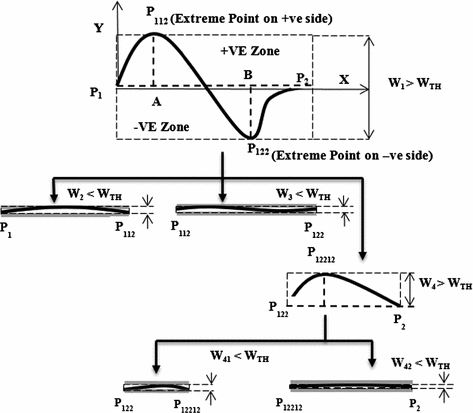
\includegraphics[width=0.495\textwidth]{images/thickedge_algorithm}
    \caption{Thick-Edge Polygonal Approximation Algorithm}
    \label{fig:thickedge_algorithm}
\end{figure}

The algorithm begins with an ordered list of points. First, a line is drawn between the first and last points, or
endpoints, of the current list of points, given by line \textbf{X} in figure \ref{fig:thickedge_algorithm}.  This can be
thought of as a potential edge in the final approximated polygon. The points are then partitioned into two sets, based
on whether they are above or below the line. Then, in each partition, the points furthest from the line, the extreme
points, are found. These are given by the points $\mathbf{P_{112}}$ and $\mathbf{P_{122}}$ in figure
\ref{fig:thickedge_algorithm}.

Then, the distance from the extreme points in each partition to the line are computed. These distances are given by
$\mathbf{A}$ and $\mathbf{B}$ in figure \ref{fig:thickedge_algorithm}. The thickness is then defined as the sum of these
two distances. If this thickness is below the user defined threshold, then we mark the endpoints as dominant points and
discard the rest of the points in the list. Otherwise, we partition the points into three sets, and then recursively
approximate each of these smaller polylines. The three partitions are from the starting point to the first extreme
point, then the first to second extreme point, and the second extreme point to the ending point, inclusive. In figure
\ref{fig:thickedge_algorithm}, the partitions would be from point $\mathbf{P_1}$ to $\mathbf{P_{112}}$,
$\mathbf{P_{112}}$ to $\mathbf{P_{122}}$, and $\mathbf{P_{122}}$ to $\mathbf{P_2}$. The algorithm terminates when no
points remain to be processed.

When there are fewer than three points in the polyline, no processing needs to be done, as all points are dominant
points by definition. The algorithm must also handle the case when there is only one extremum, as pictured by the
$\mathbf{P_{122}}$ to $\mathbf{P_2}$ curve in figure \ref{fig:thickedge_algorithm}. In this case, all points will either
be above or below the line, so there will be only one extreme point. Thus, if the points are partitioned, there will
only be two partitions, instead of three as in the usual case. Since the partitions are inclusive, a point can be marked
as dominant more than once, so the algorithm must be able to deal with duplicates. For our implementation, we use an
ordered set, which is necessary as the ordering of the points must be preserved to get an equivalent polygon.

The computational complexity of thick-edge polygonal approximation is given by equation \ref{eq:thickedge_complexity},
where $n$ is the number of points in the polygon and $a$ is the factor by which the points are partitioned, on average.
From the Master Theorem, the solution to this recurrence is $\mathcal{O}(n \log{n})$. Thus, this algorithm is very fast,
as $n$ is at most on the order of several thousand points.

\begin{equation}
	\begin{split}
		T(1) &= \mathcal{O}(1) \\
		T(n) &= n + a T \left( \frac{n}{a} \right), \quad 0 < a \leq 3
    \end{split}
    \label{eq:thickedge_complexity}
\end{equation}

%-----------------------------------------------------------------------------------------------------------------------
% Results
%-----------------------------------------------------------------------------------------------------------------------

\section{Results}

\subsection{MPEG-7 Shape Dataset}

\begin{figure}
    \centering
    \begin{subfigure}[t]{0.15\textwidth}
        \centering
        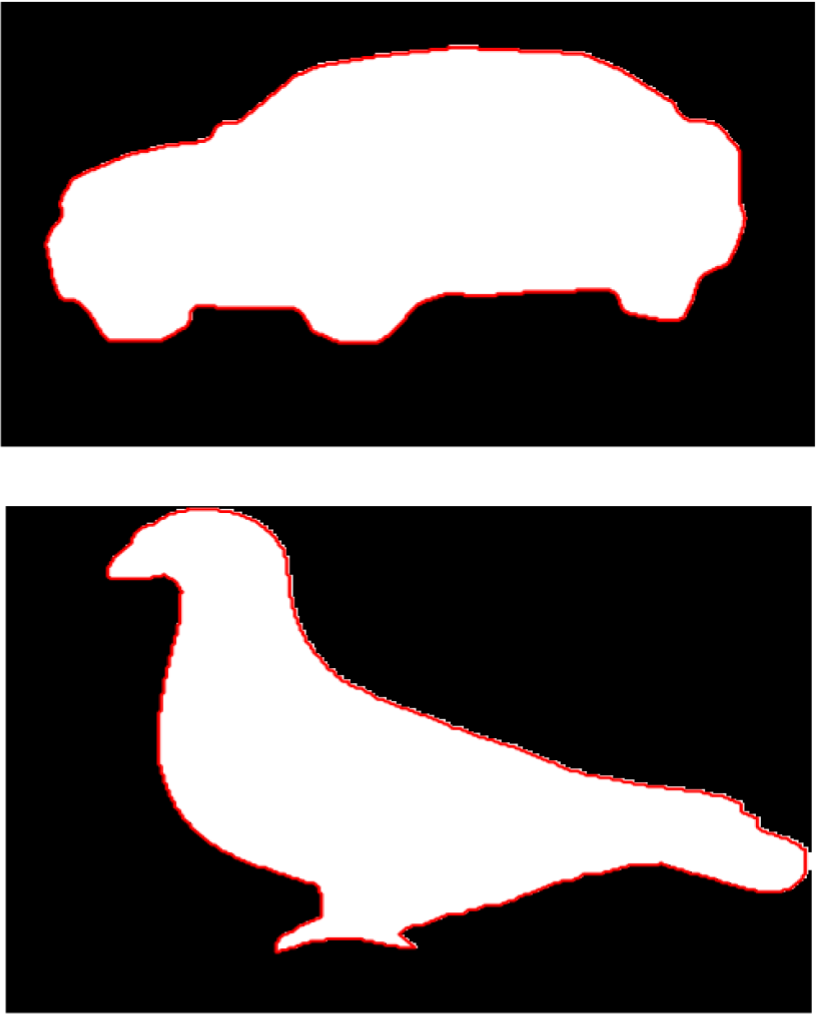
\includegraphics[width=\textwidth]{images/shape_truth}
        \caption{Original complex polygon}
    \end{subfigure}
    \hfill
    \begin{subfigure}[t]{0.15\textwidth}
        \centering
        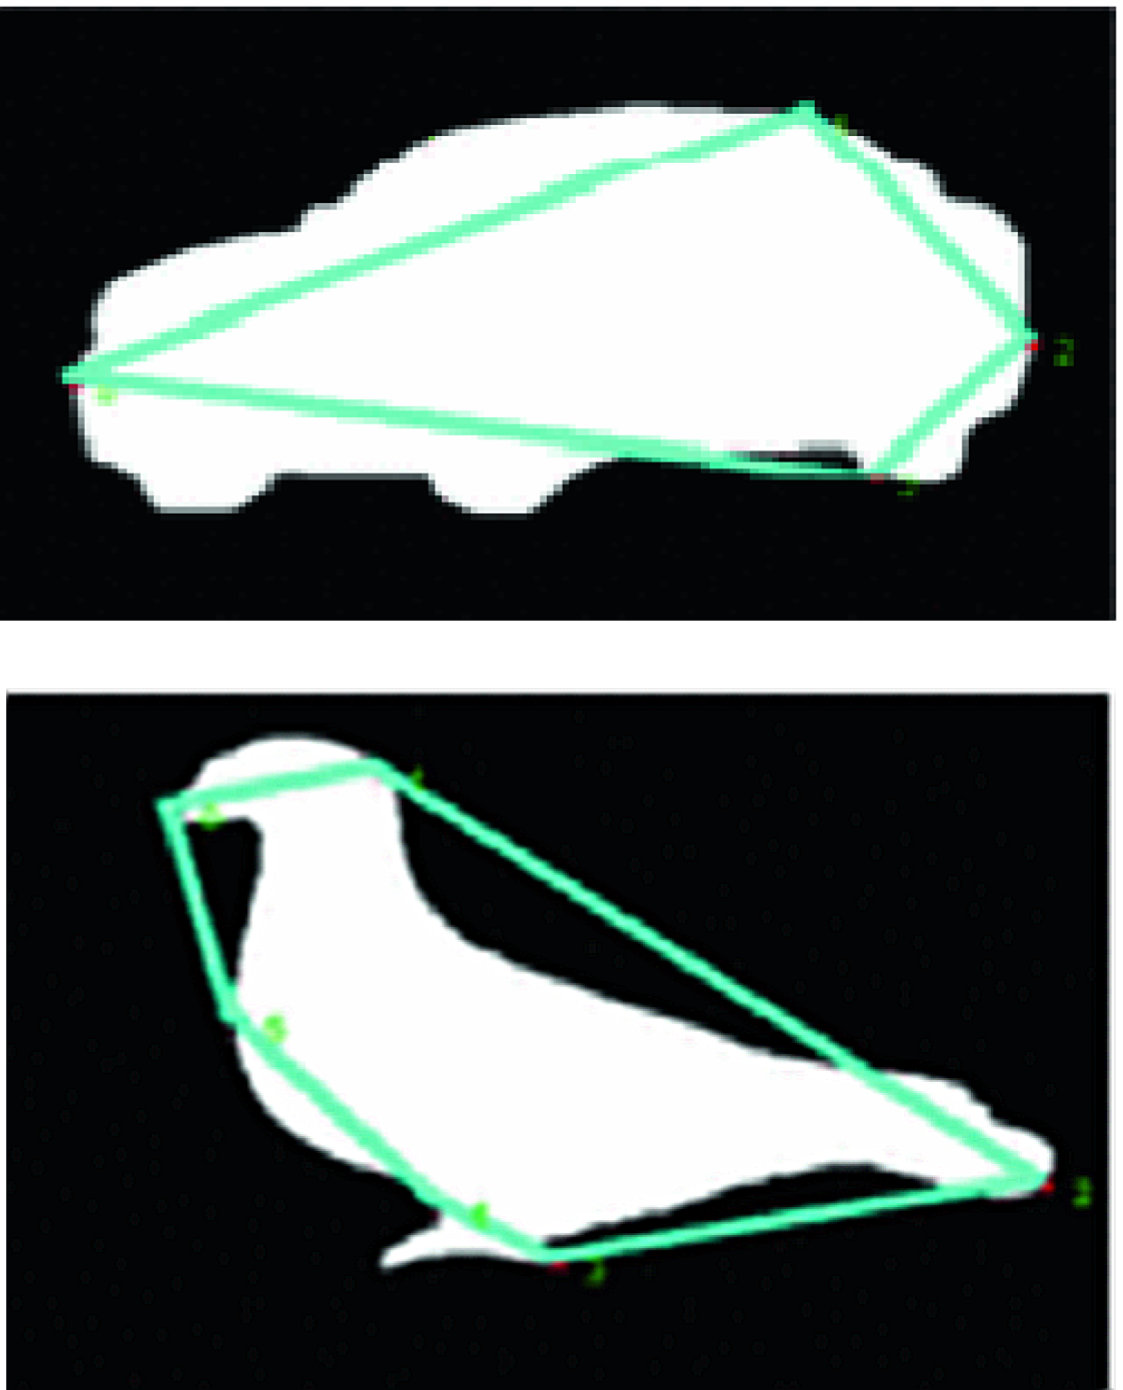
\includegraphics[width=\textwidth]{images/shape_bad}
        \caption{Ramer-Douglas-Peucker}
    \end{subfigure}
    \hfill
    \begin{subfigure}[t]{0.15\textwidth}
        \centering
        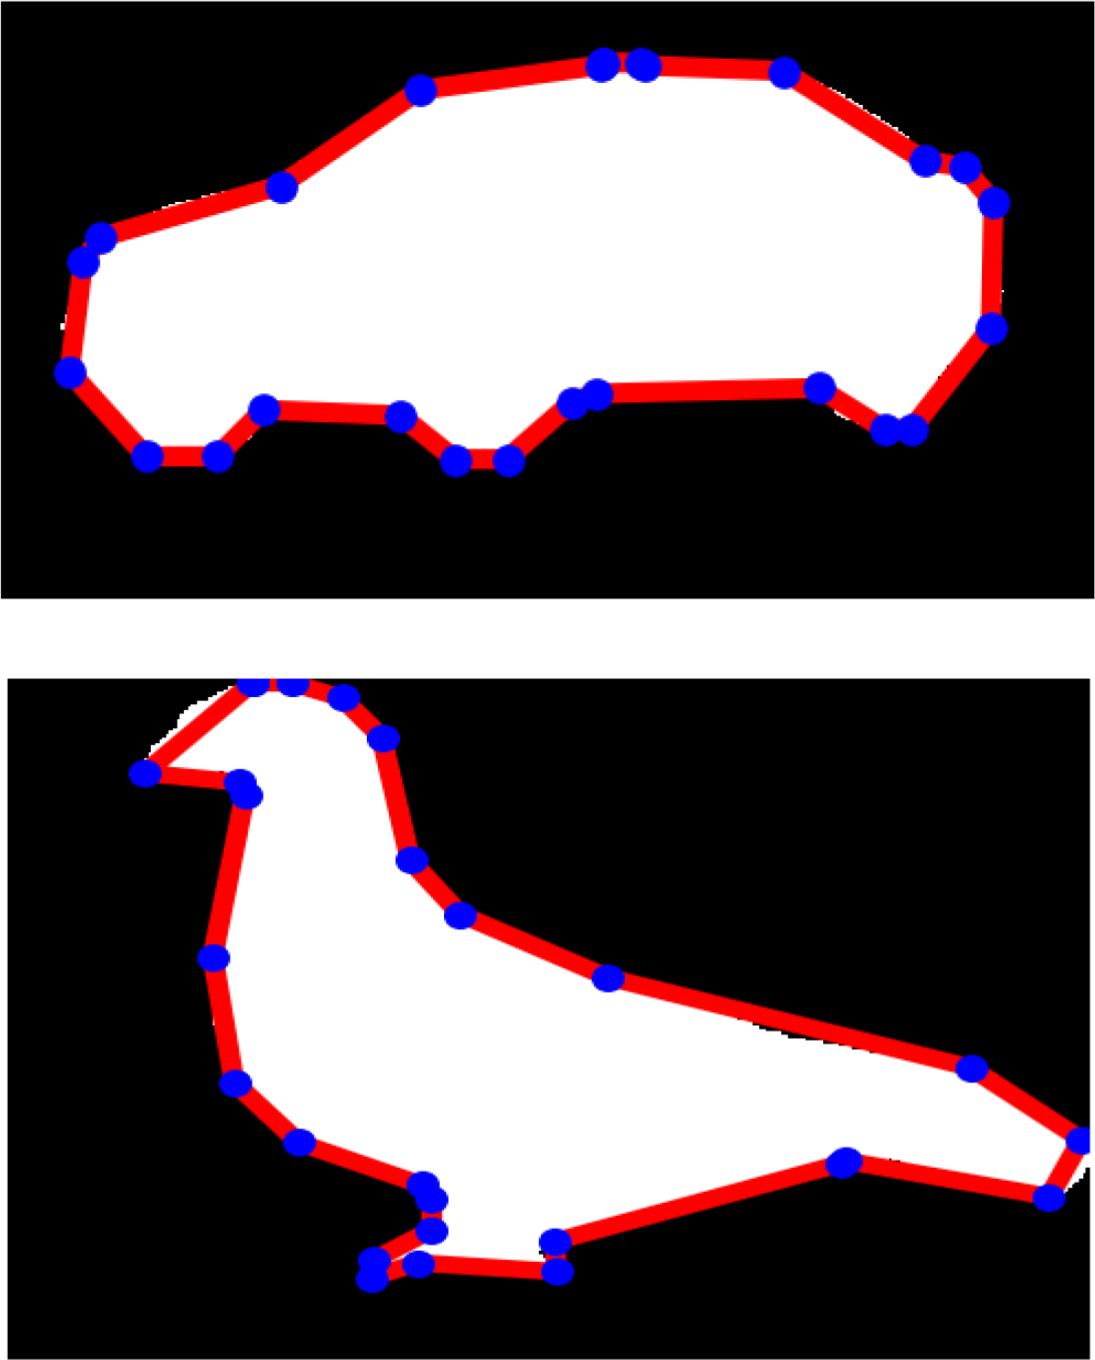
\includegraphics[width=\textwidth]{images/shape_good}
        \caption{Thick-edge}
    \end{subfigure}
    \caption{Contours on the MPEG-7 Shape Dataset}
    \label{fig:mpeg7_shape}
\end{figure}

\begin{figure*}
	\centering
    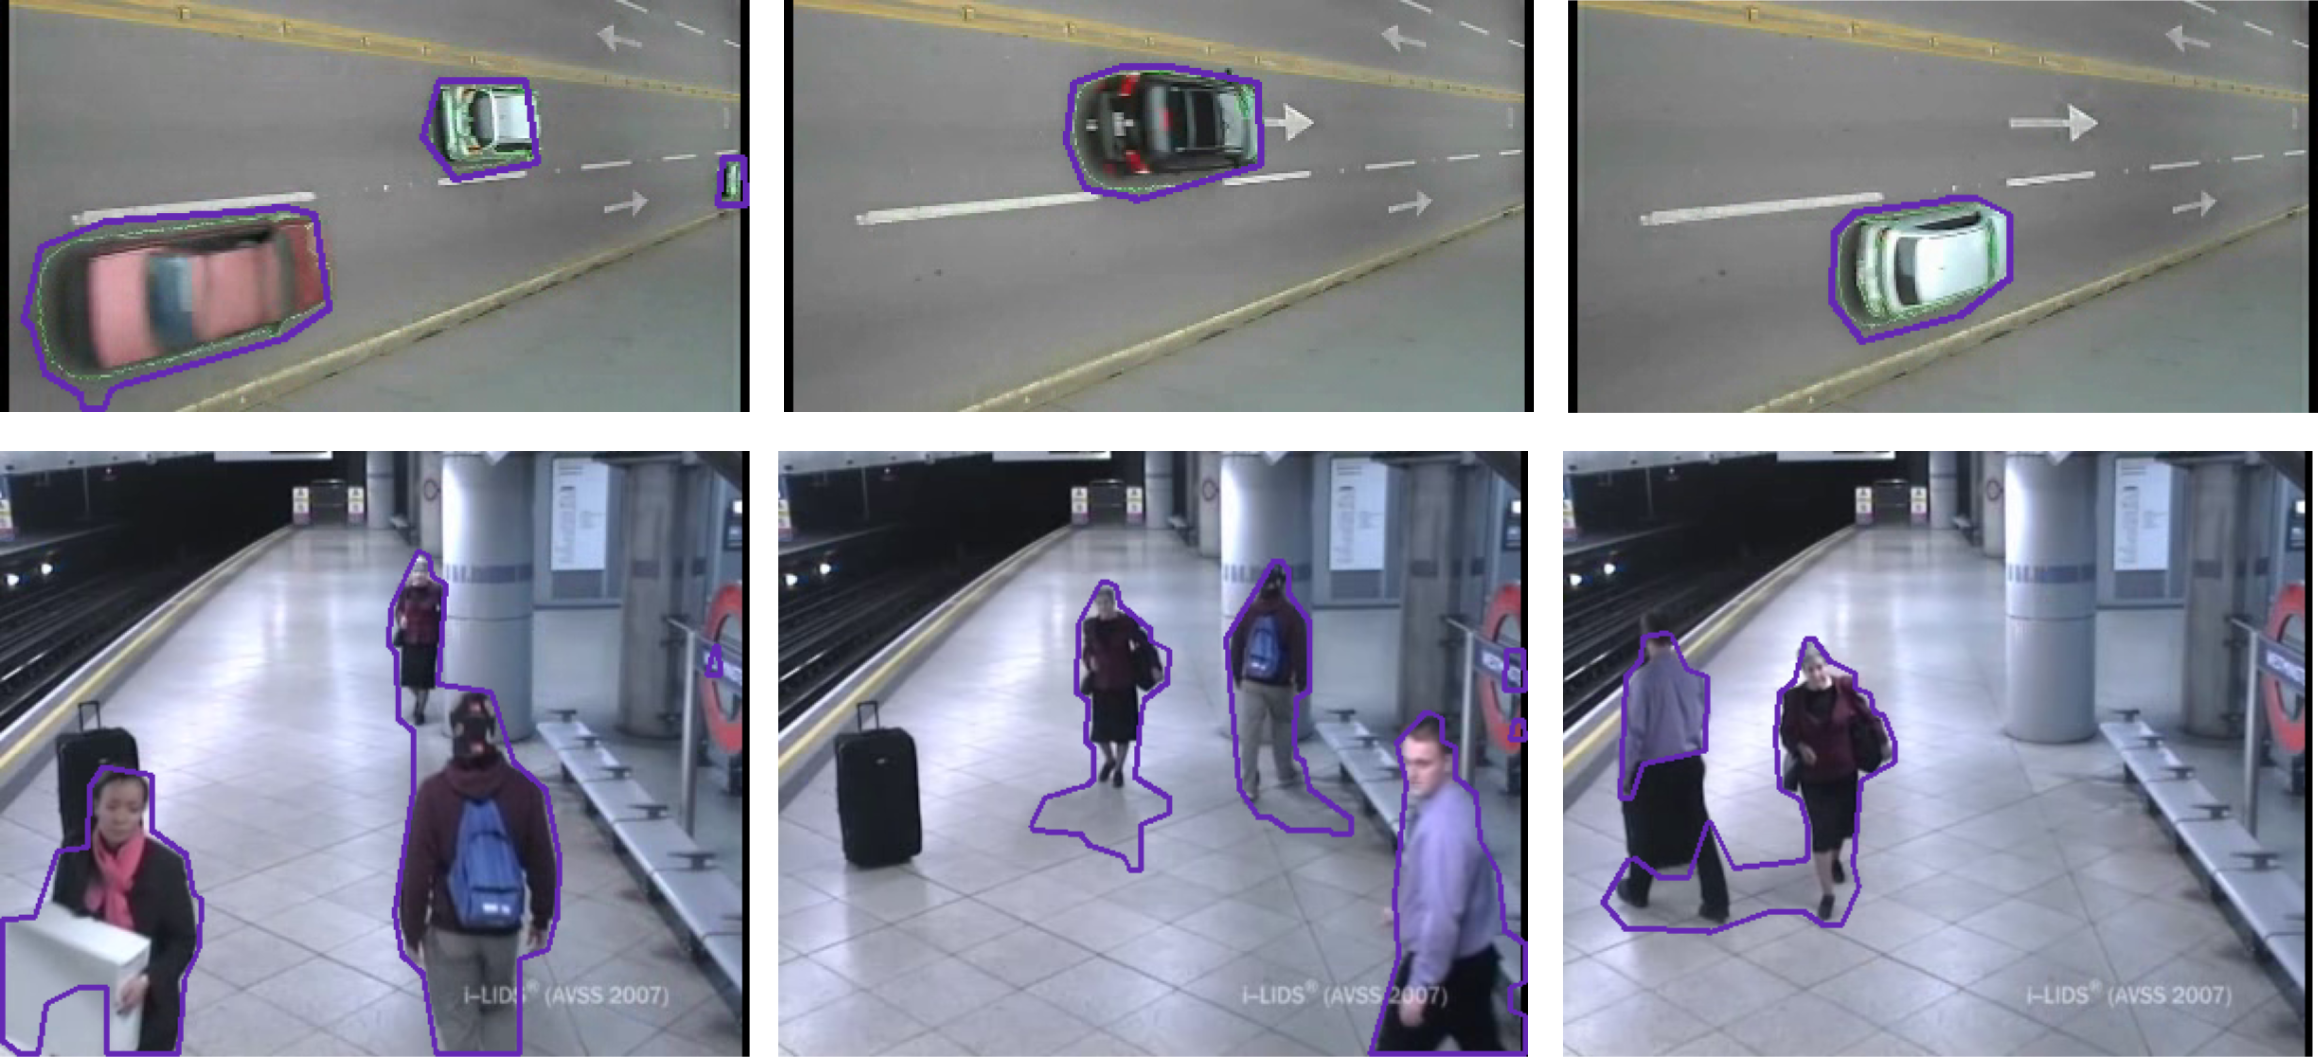
\includegraphics[width=0.95\textwidth]{images/surveillance_results}
    \caption{Example frames from two sequences: top is a car sequence, bottom is at a train station.}
    \label{fig:surv_results}
\end{figure*}

For evaluating the thick-edge polygonal approximation, we used the same dataset that was used in the Saha et al.
\cite{Saha2017} paper. This is the MPEG-7 Shape dataset \cite{MPEG-7}. This is a dataset of several thousand black and
white images that contain a single object, which is marked with white pixels. To evaluate, we simply had to trace the
contour around the image, and then feed these points into the approximation algorithm.

In figure \ref{fig:mpeg7_shape}, we show the differences between the various contours. On the leftmost column is the
polygon given when we find the contour of the edge detected image. The middle column is the resulting polygon from
Ramer-Douglas-Peucker approximation algorithm. The rightmost column is the resulting polygon from the thick-edge
approximation algorithm. The results of the Ramer-Douglas-Peucker algorithm were taken from the Saha et al
\cite{Saha2017} paper. A corresponding epsilon value for the chosen thickness parameter was used for the
Ramer-Douglas-Peucker algorithm. As can be seen in the figure, the thick-edge poylgon approximation performs far better
than the older algorithm.

For evaluation, we looked at two metrics to determine the effectiveness of the approach, the area percentage difference,
and the vertex percentage difference. The area difference captures how much information was lost by the approximation,
while the vertex difference captures how effective the compression was for the approximation. These two are given by
equations \ref{eq:vertex_difference} and \ref{eq:area_difference}, respectively, where $V'$ is the number of vertices in
the approximated polygon and $A'$ is the area of the approximated polygon.

\begin{equation}
	\text{Vertex Difference Percentage} = \frac{|V' - V|}{V} \cdot 100
    \label{eq:vertex_difference}
\end{equation}
\begin{equation}
	\text{Area Difference Percentage} = \frac{|A' - A|}{A} \cdot 100
    \label{eq:area_difference}
\end{equation}

Over the entirety of the MPEG-7 shape dataset \cite{MPEG-7}, the thick-edge polygonal approximation yielded an average
area difference of \textbf{1.31\%} and an average vertex difference of \textbf{84.86\%}. Thus, we were able to reduce
the number of vertices by 84.86\% on average, while only having an average difference of 1.31\% of the area of the
resulting polygon. For the evaluation over this dataset, we used an adaptive thickness, which was 1\% of the smallest
image dimension.

\subsection{Surveillance Footage}

Results shown in Figure \ref{fig:surv_results} are the final results of the pipeline on the surveillance data. In the
car sequence, the individual cars are easily distinguished and shown in simple but tight polygons. In the case of the
people, individuals are not distinguished in some cases as their shadow may cause a false impression that it is part of
their body. This is because the background subtraction looks for moving contiguous regions and the preprocessing
attempts to fill in all holes. Therefore, the first and last images of the train sequence fails in that it connects the
two people by their shadows.

The area the algorithm excels in is forming tight bounding polygons to the pedestrians in Figure \ref{fig:surv_results}.
Even though they move and the shape of their body changes, there is always a tight, simple bounding polygon on the order
of 10s of vertices.

\subsection{Live Video}

\begin{figure*}
    \centering
    \begin{subfigure}[t]{0.23\textwidth}
        \centering
        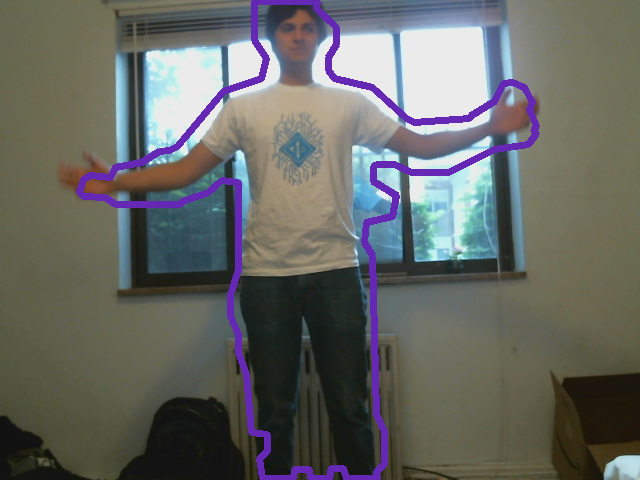
\includegraphics[width=\textwidth]{images/live_video1}
    \end{subfigure}
    \begin{subfigure}[t]{0.23\textwidth}
        \centering
        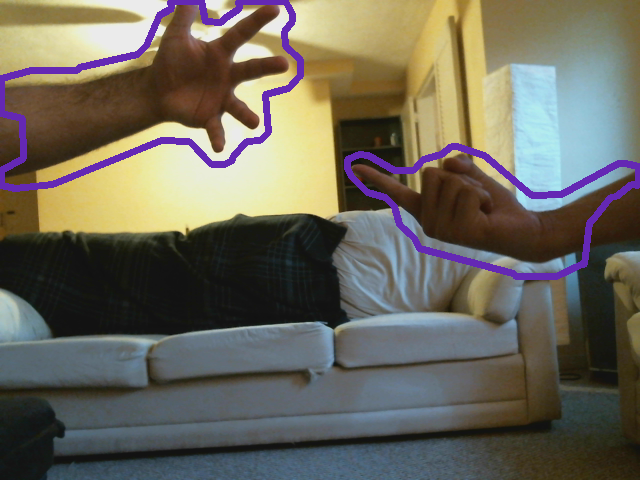
\includegraphics[width=\textwidth]{images/live_video2}
    \end{subfigure}
    \begin{subfigure}[t]{0.23\textwidth}
        \centering
        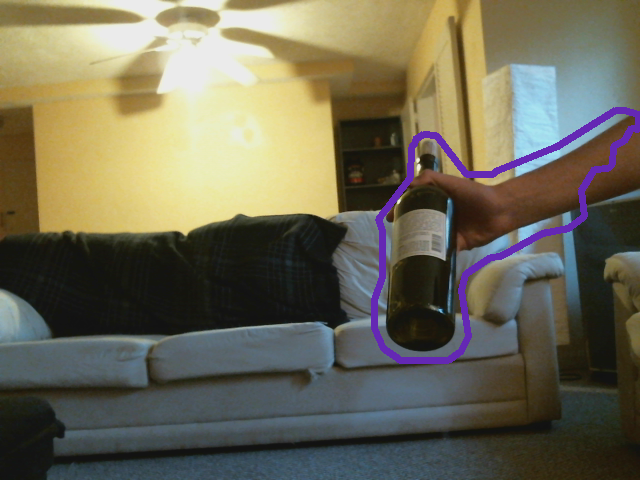
\includegraphics[width=\textwidth]{images/live_video3}
    \end{subfigure}
    \begin{subfigure}[t]{0.23\textwidth}
        \centering
        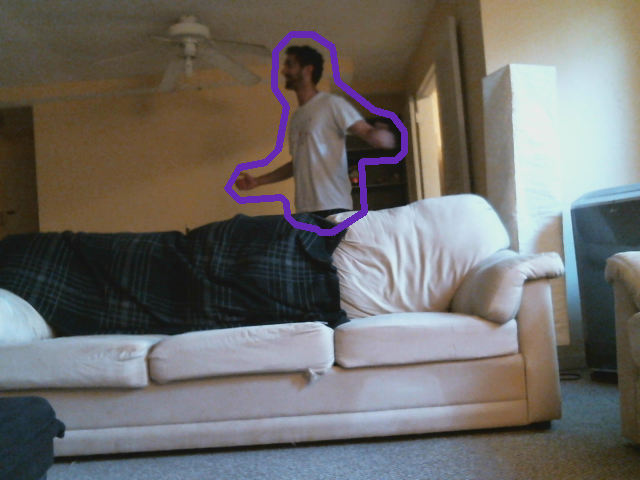
\includegraphics[width=\textwidth]{images/live_video4}
    \end{subfigure}
    \caption{Demonstration of live video from a webcam. Objects such as the wine bottle are outlined tightly and
            maintain shape information. Hands are also a good example of this. When walking, a human body's
            deformations are also captured well by the algorithm.}
    \label{fig:live_video}
\end{figure*}

Live video from the webcam was captured at 640x480 resolution and fed into the contour extraction pipeline. The video
was given a few seconds to stabilize on only a background before an actor or object was placed in the scene. The contour
of the object was approximated by a thick edge polygon of thickness of 5 pixels. In Figure \ref{fig:live_video}, we see
examples of soft bodies in the moving people as well as the hands changing shapes, and rigid bodies in the form of the
wine bottle. In all of these examples, the algorithm maintains a tight fit of a simple polygon.

%-----------------------------------------------------------------------------------------------------------------------
% Conclusions
%-----------------------------------------------------------------------------------------------------------------------

\section{Conclusions}

The thick-edge polygon approximation performs much better than the Ramer-Douglas-Peucker approximation and keeps more
information than just a bounding rectangle. As is seen in the MPEG-7 shape dataset in Figure \ref{fig:mpeg7_shape}, the
Ramer-Douglas-Puecker approximation performs poorly, not maintaining the area or shape of the original. The thick-edge
implementation always contains more data than just a rectangle and the tight polygon always maintains most area as seen
in Section 5.1. Computational cost for the thick polygon approximation is also very fast, allowing it to be calculated
in real time for even complex, high resolution contours. The bottleneck in this case is the background subtraction
library, for which the more complex algorithms take a significant time to compute. With our resolution of 640x480,
however, we still were able to maintain around 30 frames per second and therefore had a real-time implementation.

%-----------------------------------------------------------------------------------------------------------------------
% Future Work
%-----------------------------------------------------------------------------------------------------------------------

\section{Future Work}

As discussed in the motivation section, our purpose for using polygonal approximation is to use in an augmented tracking
algorithm, such as the ones proposed by Yilmaz et al. \cite{Yilmaz2004} and Liu et al. \cite{Liu2006}. The next step
would be to integrate the polygonal approximation into an object tracking pipeline to improve tracking. Future work
should also examine different background subtraction algorithms for moving cameras. This method worked very well for
stationary surveillance cameras, but there could be a demand for polygon approximation in moving cameras. This can
perhaps be done via different background subtraction algorithms and tracking.

Another item to look at is using adaptive thickness thresholds. In the thick-edge polygonal approximation algorithm, the
thickness is hand selected by the user, but it is possible that it could be automatically selected. One approach, which
was explored briefly in the results, was to make the threshold a percentage of the image dimensions. Another idea would
be to use the area of the original polygon to determine the threshold. The idea would be to look at the ratio of the
area of the object's bounding box to its polygon. If this ratio is large, then the object is close to rectangle, so it
is less likely it will have many bumps in its contour, so a larger threshold can be used. Otherwise, if the ratio is
small, the object will potentially have a more complex contour, so a smaller threshold should be used.

%-----------------------------------------------------------------------------------------------------------------------
% Division of Work
%-----------------------------------------------------------------------------------------------------------------------

\section{Division of Work}

Brandon Perez worked on the thick-edge implementation in NumPy. He researched the topic and analyzed the performance of
various algorithms to create a fast, real-time implementation of the original paper. He ran this on the MPEG-7 detaset
to have quantitative data on the performance and to verify the implementation. He also worked on the live webcam feed
and designed the live demo.

Sohil Shah worked on the background subtraction pipeline. He analyzed the various algorithms implemented in Sobral's
paper and chose the best one for the targeted application. He worked on the preprocessing pipeline using NumPy and
OpenCV and designed a robust method to extract contours from binary images. He also analyzed the full implementation
against surveillance datasets to determine the best parameters.

%-----------------------------------------------------------------------------------------------------------------------
% References
%-----------------------------------------------------------------------------------------------------------------------

{\small
	\bibliographystyle{ieee}
	\bibliography{references}
}

\end{document}
